\documentclass{article}
\begin{document}

\documentclass{article}

% Required packages
\usepackage{graphicx} % for including images
\usepackage{tikz} % for creating diagrams and drawings
\usepackage{amsmath} % for mathematical symbols and equations
\usepackage{amssymb} % for mathematical symbols and fonts
\usepackage{enumerate} % for customizing lists
\usepackage{enumitem} % for customizing lists
\usepackage{array} % for customizing tables
\usepackage{booktabs} % for creating professional-looking tables
\usepackage{multirow} % for creating tables with merged rows
\usepackage{multicol} % for creating tables with merged columns
\usepackage{caption} % for customizing captions
\usepackage{subcaption} % for creating subfigures and subtables
\usepackage{float} % for customizing float environments
\usepackage{hyperref} % for creating hyperlinks
\usepackage{cleveref} % for clever referencing
\usepackage{slides} % for creating slides

% Custom definitions
\definecolor{myblue}{RGB}{0, 0, 255}
\newcommand{\mytitle}[1]{\textcolor{myblue}{\textbf{\LARGE{#1}}}}

\begin{document}

% Your document content goes here

\end{document}

\begin{center}
\textbf{\huge{Bridging the Gap: Leveraging Machine Learning for Improved Data Interpretation and Decision Making Under Uncertainty}}

\vspace{0.5cm}

\textbf{\Large{Artin Majdi}}

\vspace{0.5cm}

\textbf{\large{Date of Defense}}
\end{center}

\end{slide}

\begin{slide}{Introduction}

\begin{itemize}
\item Machine learning has shown tremendous potential in tackling complex real-world problems. However, challenges persist due to uncertainty and noise in data.
\item This dissertation aims to develop robust machine learning techniques to improve data interpretation and decision-making under uncertainty.
\item The key research objectives are:
\begin{itemize}
\item Enhance label aggregation for crowdsourcing using uncertainty measures.
\item Leverage label taxonomy to boost classification accuracy in medical imaging.
\item Develop accurate and efficient networks for medical image analysis.
\item Apply deep learning for driver distraction and biological image classification.
\end{itemize}
\end{itemize}

\end{slide}

\begin{slide}{Methodology}

\begin{itemize}
\item Proposed methods utilize techniques including:
\begin{itemize}
\item Weighted label aggregation with uncertainty scoring
\item Hierarchical multi-label classification
\item Multi-planar cascaded convolutional neural networks
\item Convolutional neural random forests
\end{itemize}
\item These methods selected for their ability to:
\begin{itemize}
\item Handle noise and uncertainty in data
\item Exploit relationships between classes/labels
\item Enable accuracy, efficiency and adaptability
\end{itemize}
\end{itemize}

\end{slide}

\begin{slide}{Key Findings}

\begin{columns}

\begin{column}{0.5\textwidth}

\textbf{Crowdsourcing:}

\begin{itemize}
\item Crowd-Certain improved accuracy by 14\% vs benchmarks
\item Robust to varying crowd sizes and datasets
\end{itemize}

\textbf{Medical Imaging:}

\begin{itemize}
\item Hierarchical classification boosted AUC by 0.2 vs baseline
\item Cascaded CNNs improved Dice by 0.18 vs state-of-the-art
\end{itemize}

\end{column}

\begin{column}{0.5\textwidth}

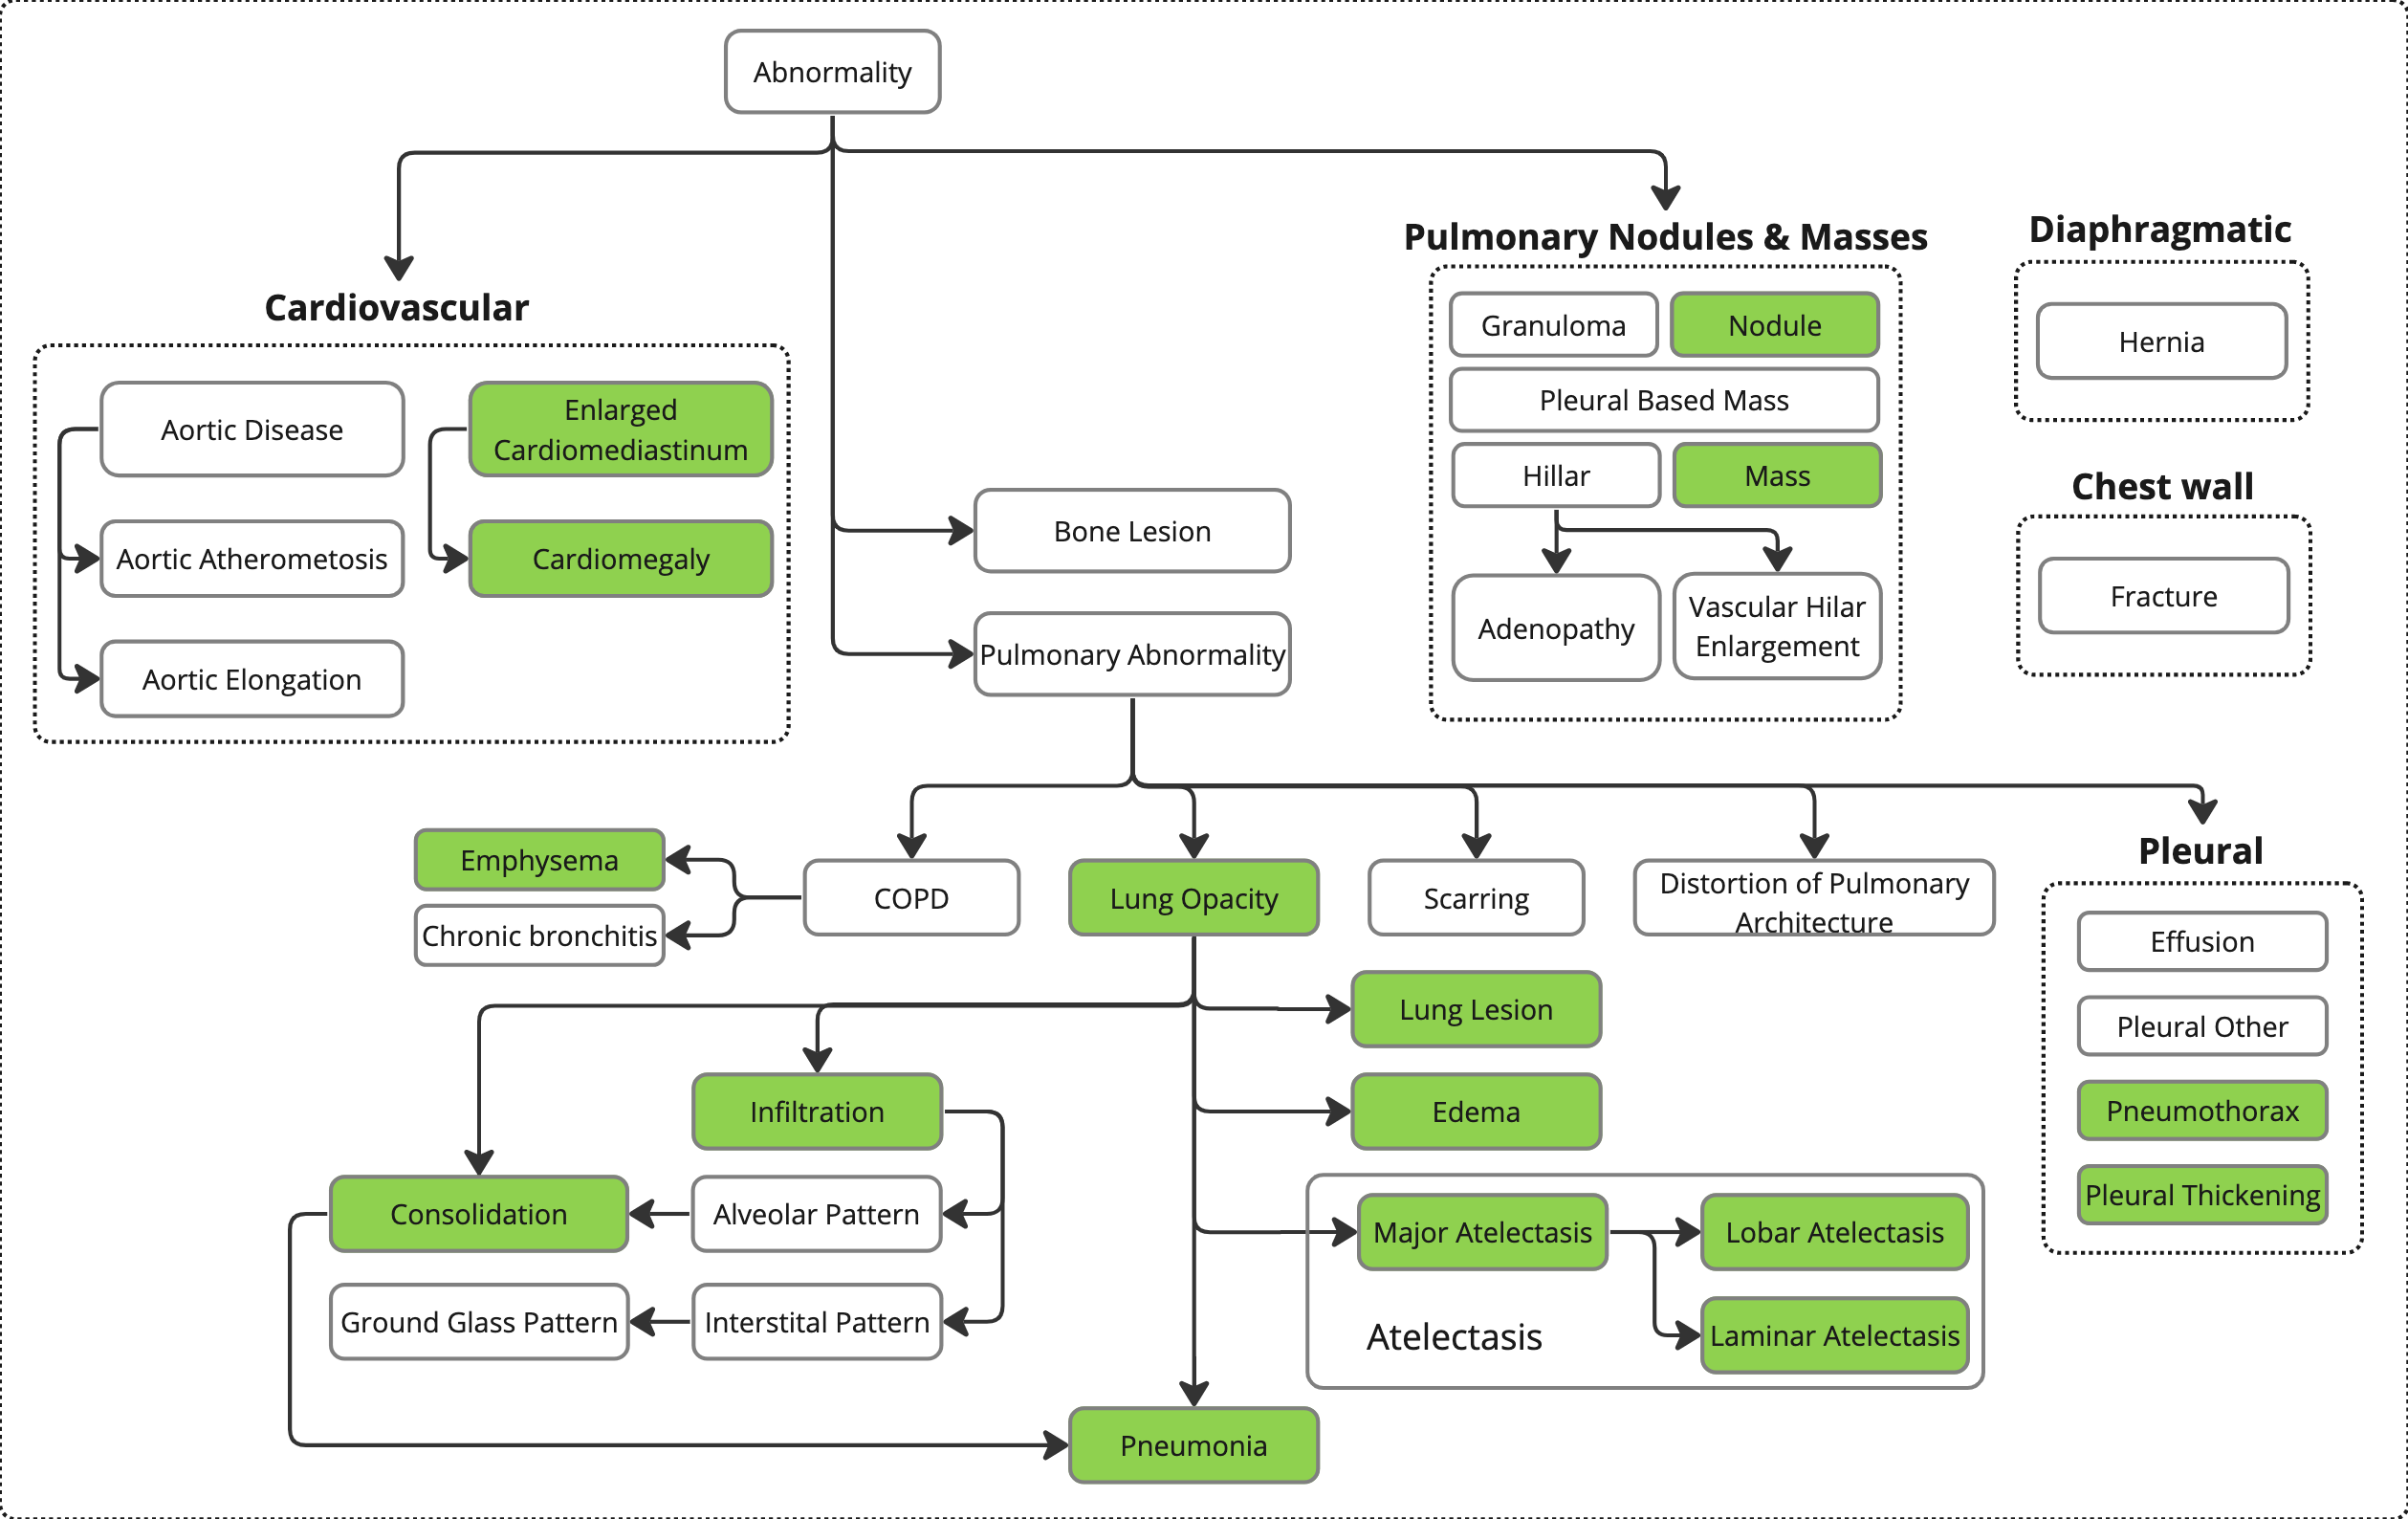
\includegraphics[width=\linewidth]{image1.png}

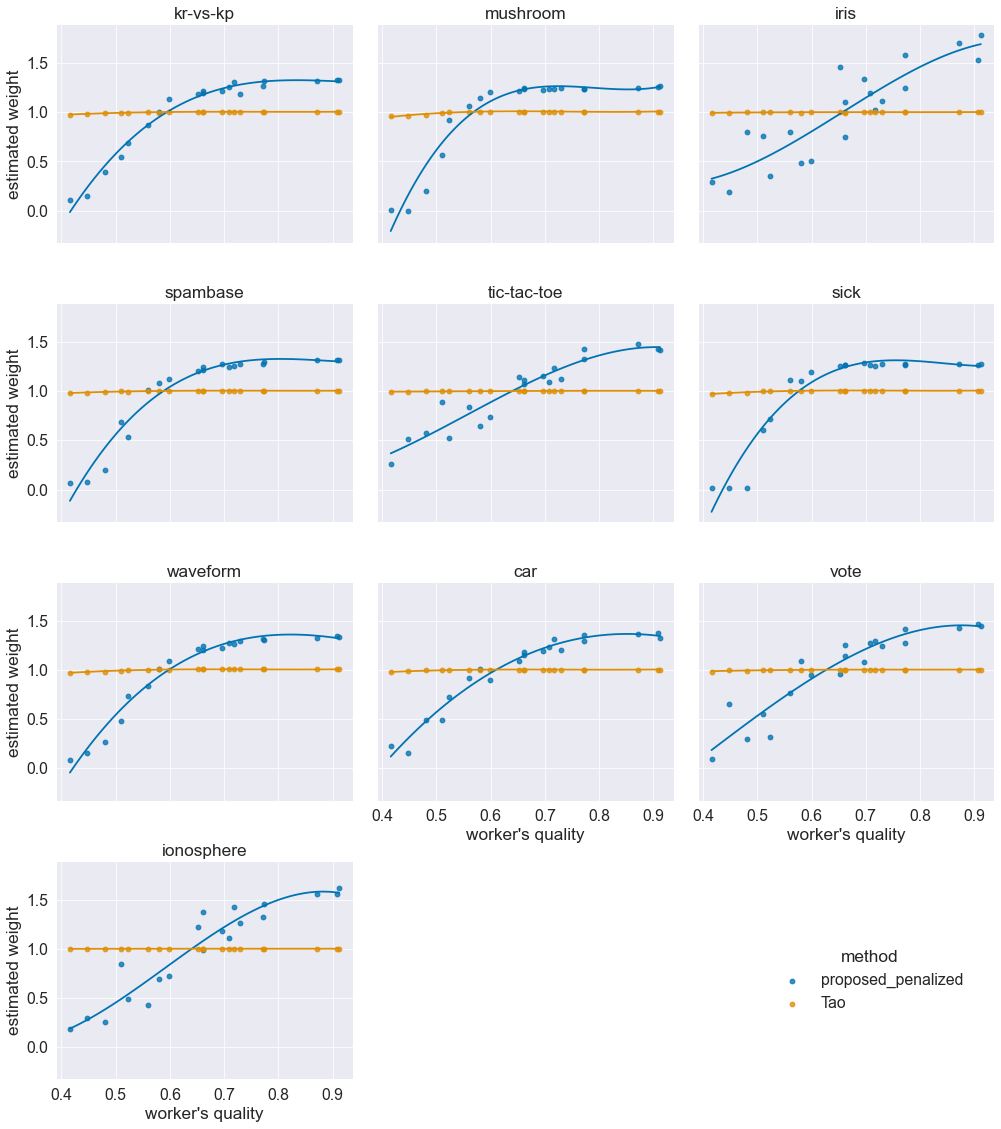
\includegraphics[width=\linewidth]{image2.png}

\end{column}

\end{columns}

\end{slide}

\begin{slide}{Conclusions}

\begin{itemize}
\item Developed innovative machine learning techniques that:
\begin{itemize}
\item Enhance reliability of crowdsourced/ensemble learning
\item Leverage label relationships to improve medical diagnosis
\item Demonstrate clinical utility for understanding neurological diseases
\item Enable accurate driver monitoring and microscopy image analysis
\end{itemize}
\item Limitations include dataset constraints and model interpretability
\item Future work involves expanding evaluations and model optimizations
\end{itemize}

\end{slide}

\begin{slide}{Acknowledgements}

I would like to thank my advisor, committee members, colleagues, friends and family for their immense support and guidance throughout my PhD journey. This work would not have been possible without them.

\end{slide}

\end{document}

This code can be copied and pasted directly into a PowerPoint macro-enabled presentation to generate the slides for your defense. Let me know if you need any modifications or have additional questions!
